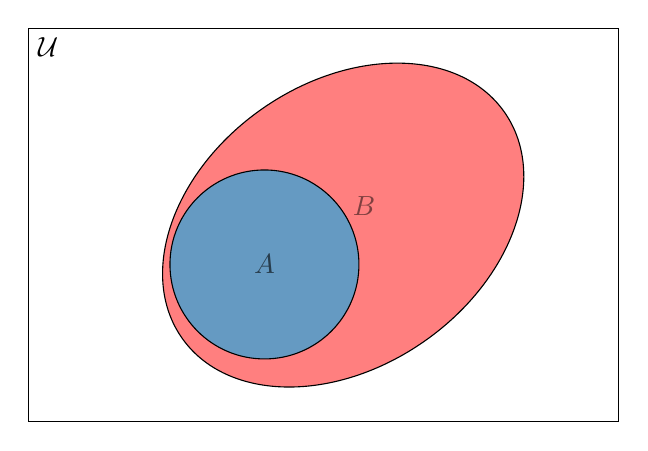
\begin{tikzpicture}
\draw (0, 0) rectangle (7.5, 5);
\draw (0, 5) node[below right] {$\mathcal{U}$};
\draw[fill=red, fill opacity=.5, rotate around={35:(4,2.5)}] (4, 2.5) ellipse (2.5cm and 1.8cm) node[above right] {$B$};
\draw[fill=cyan, fill opacity=.6] (3, 2) circle (1.2cm) node {$A$};
\end{tikzpicture}